\documentclass[11pt, fleqn]{article}

\usepackage[margin=.75in]{geometry} 
\usepackage{amsmath,amsthm,amssymb}
\usepackage{pgfplots}
\usepackage{tikz}
\usepackage{enumerate}
\usepackage{graphicx}
\usepackage{subcaption}
\usepackage[font=small]{caption}
\usepackage[compact]{titlesec}

\begin{document}

\title{\vspace{-2cm}Project Midterm Report}
\author{Cean Park (ckp42), Tiffany Shih (ts568)\\
ORIE 4741: Learning with Big Messy Data \\ October 27, 2017}
\date{}

\maketitle

\vspace{-1cm}
\section{Project overview} 
The topic of our study is The New York State Tuition Assistance Program (TAP), New York's largest financial aid grant program. Eligible residents of New York State that attend in-state colleges or universities can apply for the TAP to help pay for their tuition. According to New York’s Higher Education Services Corporation (HESC), students may apply for the TAP through the FAFSA, and the award amount is determined by various factors including the academic year in which the first payment of TAP is received, the type of postsecondary institution attended, taxable income, and financial status. 

The goal for our project is to build a model that can accurately predict an applicant's TAP grant award amount given a set of data from his/her TAP application. Through our data analysis, we hope to determine which fields from a TAP application have the greatest impact on award decisions as well as observe any trends or patterns that have been present in applications since the year 2000. Given that the NYS HESC provides a TAP Award Estimator tool on their site, we may also try to compare our results to the online tool and see how our predictions differ.

\section{About the data}

\subsection{Data set overview}
The data set we are using to complete our analysis is provided by the New York State government. It examines Tuition Assistance Program (TAP) Recipients \& Dollars by Income, Age Group and Program Information for the academic years 2000 to 2015. The data set contains 190,964 examples across 16 features, and stratifies recipients by various factors including age, academic level, type of institution, and financial status. For each stratum, the data set lists the number of TAP recipients and FTEs (Full Time Equivalents) that fall under the aforementioned categories as well as total award amount granted to that group of recipients. In order to make a prediction for a single applicant, we defined a new output feature, ``Average Award Per FTE'', in order to provide an individual rather than aggregate award amount.

The data is composed of a combination of 9 nominal, 5 discrete, and 2 continuous features. Some of the nominal features include Institution Type, Level of Study, and TAP Sector Group. The discrete features include some of our input features, such as ``Income'', ``Year'', and ``Headcount''. Our continuous features are ``Average Award Per FTE'' and ``Average Income'', which is defined in the Data cleaning section below.

From a first glance at the data, the dependency status, age group, sector group, and income level features seem promising as significant variables for prediction.


\subsection{Data cleaning}
Our goal in cleaning the data was to transform the given TAP recipient data set into entirely numerical values for use in our preliminary model selection. Although there were only 9 nominal variables, many of the other columns in our data were parsed as string objects in the provided CSV file, and thus needed cleaning for usability.

For nominal features, we employed two types of transformations to obtain numerical data:
\begin{enumerate} [(1)]
	\item 
		For nominal features with only two categories, we created a binary column such that a value of 1 represented one category and a value of 0 the other. This was done for the “TAP Level of Study,” “Sector Type,” “TAP Financial Status,” and “Degree/Nondegree” features.
	\item
		For nominal features with more than two categories, we used one-hot encoding transform a feature with k categories into k binary-valued columns. This was applied to the other 5 nominal features.

\end{enumerate}

Although most of the discrete/continuous features were encoded as numbers in the data, the Income features were provided in the data were strings describing the range of income, e.g. ``\$2,001 to \$3,000''. We decided to numerically represent the income range as the average of the endpoints, so we wrote a function to parse each endpoint and return the average; this feature was labeled as ``Average Income''.

By using the $isna$ function, we found that the provided data set surprisingly only had two missing values, both of which were in the ``TAP Recipient FTE'' column. Since both missing values corresponded to ``Headcount'' values of 1, and each headcount can either be equal to 0.5 or 1 FTE, we replaced both empty values with the average of the two, 0.75.

Lastly, we removed the ``Headcount'', ``FTE'', and ``Dollars'' columns (since these features describe the aggregate applicant pool) and added an offset column for a total of 42 columns in our data set. We anticipate additional data cleaning and transformations to be conducted as we include different types of models in our project.

\begin{figure}
	\begin{center}
	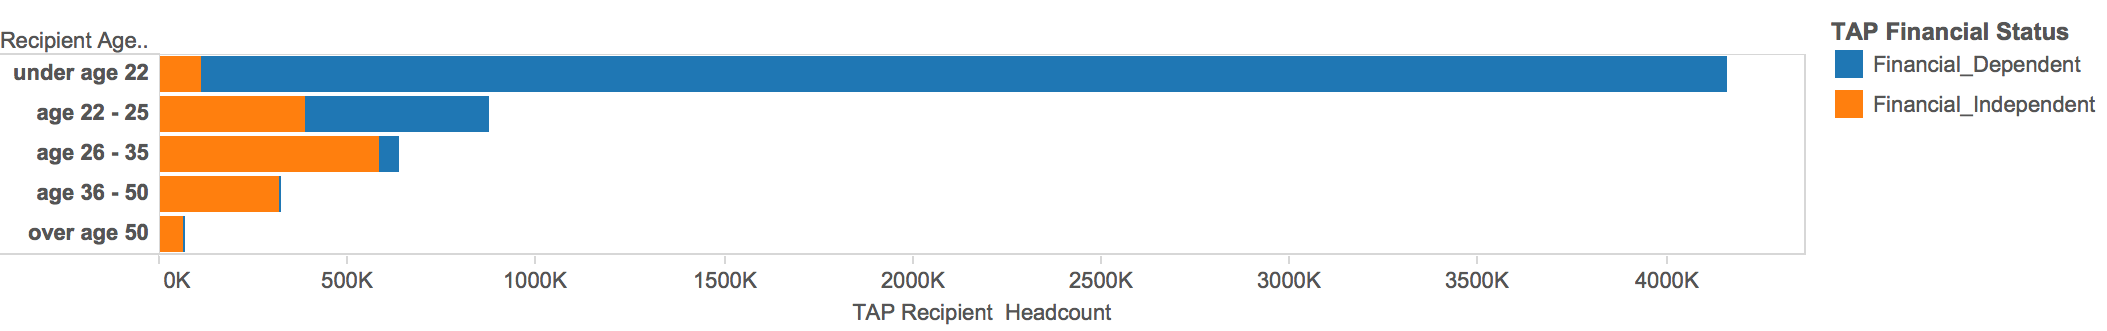
\includegraphics[scale = 0.30]{financial_status.png}
	\caption{Recipient Demographic by Age and Financial Status}
	\end{center}
	\begin{minipage}[c]{0.4\linewidth}
		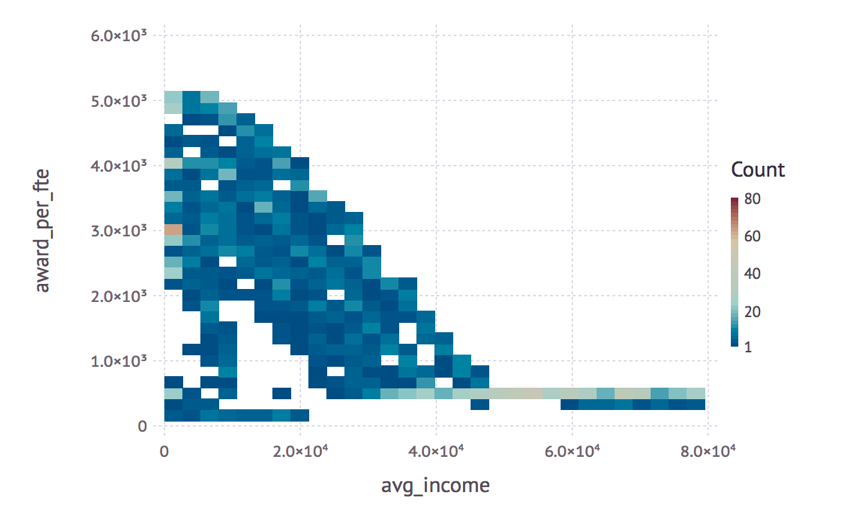
\includegraphics[width=\linewidth]{avgincome_vs_award.png}
		\caption{2-D Histogram of Grant Award per FTE vs. Income}
	\end{minipage}
	\hfill
	\begin{minipage}[c]{0.5\linewidth}
		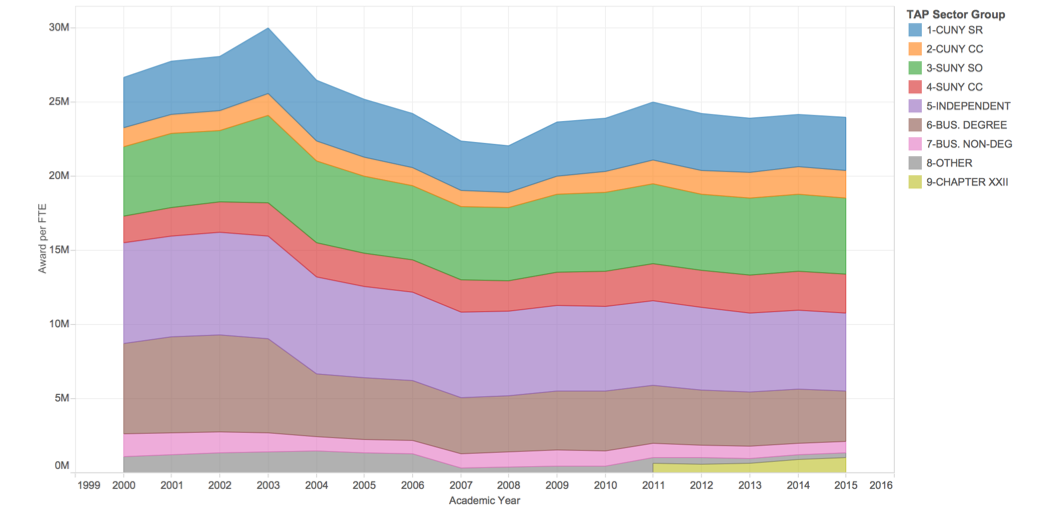
\includegraphics[width=\linewidth]{sector_group.png}
		\vspace{-0.5cm}
		\caption{Sum of TAP Awards from 2000-2015 by Sector Group}
	\end{minipage}
\end{figure}

\subsection{Exploratory data analysis}
In order to achieve a better understanding of our data, we explored various summary statistics and visualizations. First and foremost, we wanted to understand what kind of demographic we were working with (see Figure 1). It is evident through this bar graph that the major demographic of TAP recipients consists of students under the age of 22 who hold financial dependent status. This is consistent with our assumptions of the population.

In addition to demographic, we wanted to observe which variables might carry a heavier weight in the grant award decision, and intuitively, we thought that might be a recipient’s average income. Due to the vast amount of examples that we have in the data set, we took a simple random sample of 1,910 examples to generate our visualization.


From our histogram (see Figure 2), it is evident that there is some correlation between average income and grant award. In general, as average income increases, grant award decreases. However, it is interesting to note that the award granted to recipients with average income over \$50,000 is capped at around \$500, while there is great variability within the awards granted to recipients in the lower average income regime. This could indicate that there is another variable that significantly influences grant award decision, especially for low average income recipients. This is certainly something we will explore as we continue our analysis.

Another aspect of the data we were curious about was the variability of TAP awards from year to year. Plotting these (see Figure 3), it seems that there is a notable increase in total awards granted from 2000 to a peak in 2003 and a notable decrease from 2003 to a low in 2008. This low point could perhaps have been influenced by the recession of '08. We also wanted to add another dimension to this visualization to see if students enrolled in a certain category of NYS colleges/universities received more or less grant awards than others. It seems that state-operated SUNY schools as well as independent colleges receive a larger fraction of the total grant pool. 

In addition to these visualizations, a couple notable summary statistics include the mean and median grant award amounts, which are \$2,101.76 and \$2,033.33 respectively. Given that TAP recipients can be awarded up to \$5,165 annually, it seems that it is more common for recipients to receive less than half the total potential award amount. This could be due in part to the \$500 cap that we noticed for those in the upper half of the average income range.



\section{Preliminary models and evaluation}
Our preliminary analysis consisted of a few supervised models to forecast our prediction performance at a high level. To facilitate this, we partitioned our cleaned data set into training (60\%), validation (20\%), and test (20\%) sets by applying Scikitlearn's $training\_test\_split$ function twice.


\subsection{Linear regression and model effectiveness}
We first ran a simple linear regression with our cleaned, numerical data set (with offset) on all 42 features. The objective of the linear regression was to find the minimizer of $f(w) = ||y - Xw||^2$, where $y \in \mathbb{R}^{d}$ was our desired output data, $X \in \mathbb{R}^{n \times d}$ our input data with $n$ examples across $d$ features, and $w \in \mathbb{R}^{d}$.

The 42 coefficients of $w$ obtained via least-squares regression were both positive and negative and large in magnitude, ranging from a value of -24,350.4 as our offset term all the way to 4005.3 for the binary feature representing Award Schedule E. Since our predictor $y$ ranges from 0 to \$5,000, we decided to measure error via mean absolute error (MAE) and mean absolute percentage error (MAPD). The MAE and MAPD on our training, validation, and test sets are the two measurements we plan to use to test the effectiveness of our models developed moving forward.

Across the training, validation, and test sets, MAE and MAPD values were similar, around \$510 and 62\% respectively. On average, our linear model prediction was \$510 and 62\% off from the true value, which demonstrates poor performance and severe underfitting.

It may be worth considering running a regression without a few features, e.g. excluding year since the calendar year is not necessarily applicant-specific information.

\subsection{Overfitting and underfitting}
By including both a training and validation set, we hope to utilize $k$-fold cross-validation in order to detect whether our model is over/underfitting. To remedy underfitting, we will provide more features to our input data $X$, either in the form of additional feature transformations or simply constructing new columns based on existing ones. On the other hand, to remedy overfitting, we want to utilize regularizers in our models and determine optimal feature selection such that we obtain a well-fitted model.



\section{Next steps}
In order to improve our predictions and analysis moving forward, we want to use further transformations of our data (rather than our simple numerical encoding) to better portray the information in the data set. In addition, we want to develop models on subsets of the data (e.g. by year) to determine whether there exist any patterns or trends in TAP award distribution across a particular feature.

We also want to determine the best prediction model for the data, using techniques we have learned in class such as regression trees, random forest, and regularization. The ultimate goal for our project is to benchmark our best prediction model against the esimated award calculator currently provided on the NY.gov website.

\end{document}

